\newpage

\subsection{Effective implementation}

Before implementing real-time in a web application it is important to make a suitable decision if you want to use WebSockets or Server Sent-Events. This comes down to choosing between bidirectional or unidirectional communication.

A feature can be implemented in real-time in 2 different ways. In the first way the data is sent from client to server using a bidirectional connection and the other clients receive the new data from the server thus using WebSockets. The second option consists of using a HTTP request to send data to the server and updating the clients using Server Sent-Events and thus only needing a unidirectional persistent connection.

This means there is a difference between needing bidirectional communication and choosing to use it. In some use cases choosing for a HTTP request to send data is not sufficient enough and can impact the performance:

\begin{enumerate}
  \item Canvas tools: Figma, Miro
  \item Multiplayer games
  \item Text-editing
\end{enumerate}

The data that needs to be constantly transmitted can benefit from a bidirectional connection because the connection is persistent and doesn't have to be created for each change. But in other features this is not necessary and a HTTP request is sufficient for example:

\begin{enumerate}
  \item Live status boards
  \item Real-time stats
  \item Notifications
\end{enumerate}

The final thing to always keep in mind is to make sure the application is future proof. When choosing SSE there are limited options to expand with features that require bidirectional communication while choosing WebSockets from the start doesn't cause this issue. This is an important trade off that needs to be made. Choosing Server Sent-Events makes sense to keep it simple and definitely makes sense when upgrading something into real-time that was not in real-time before.

\subsubsection{WebSockets implementation}

To provide a basic example of how to use WebSockets a POC will be worked out to understand the 2 types of features. So feature 1 is using WebSockets in a setting where Server Sent-Events is sufficient but also using the same WebSocket to provide feature 2, that needs the bidirectional communication. The first feature is a status board and the second feature is a canvas with moving objects. SocketIO will be used to demonstrate the features a library can bring to the table, chosen because of its easy implementation.

\textbf{POC setup}

\begin{figure}[h]
  \caption{POC diagram}
  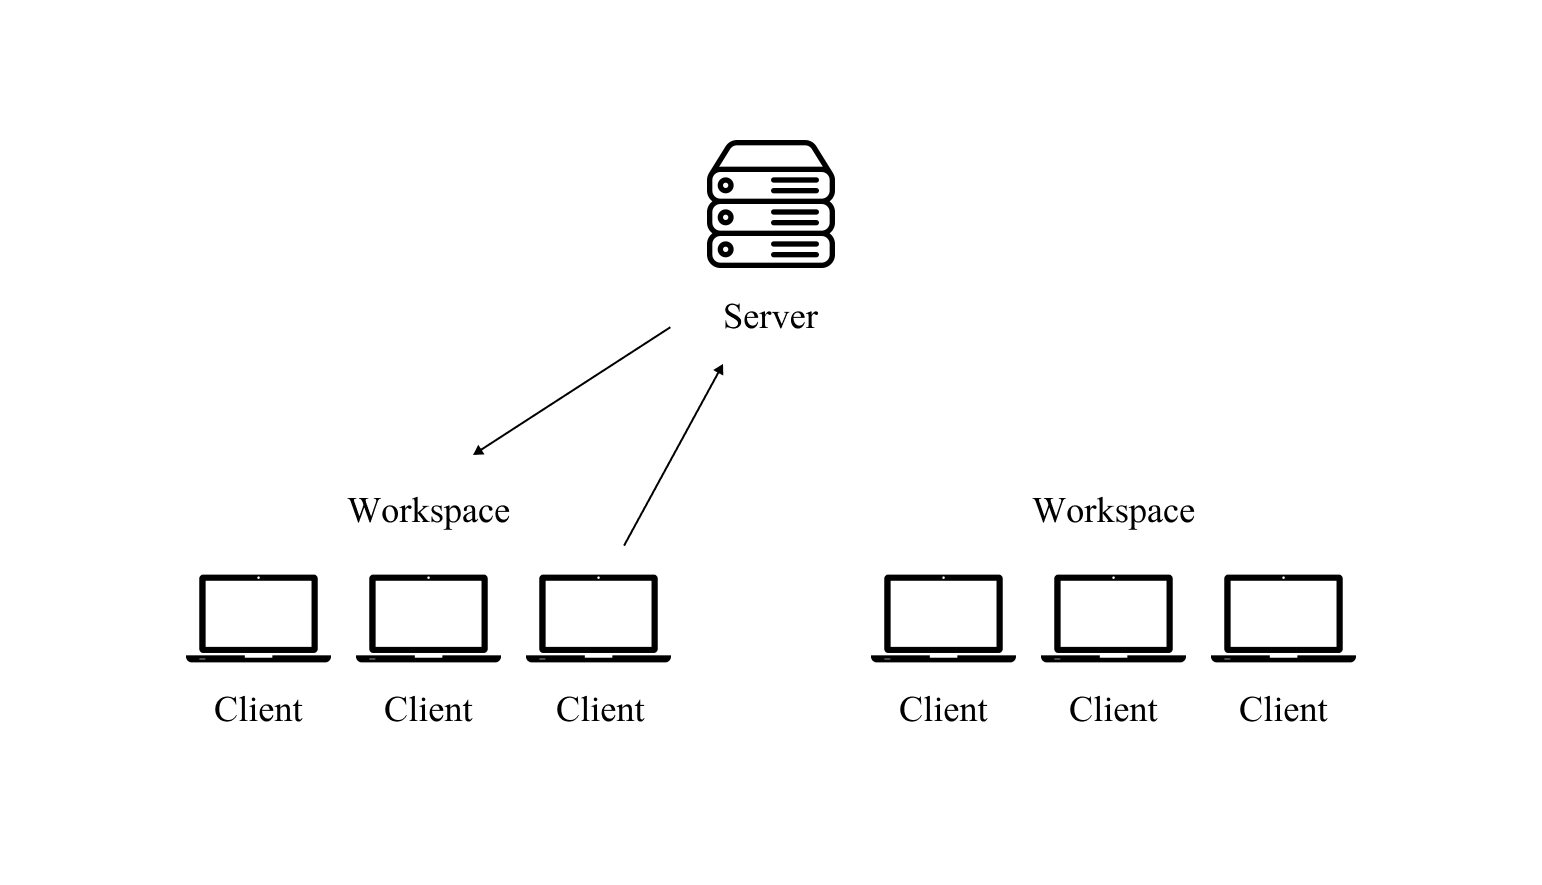
\includegraphics[width=0.8\linewidth]{POC_diagram}
  \centering
\end{figure}

Before implementing the features in this POC there are some things that need to be implemented first. A collaborative feature means different users working together, so users meaning authentication and authorization is a must have before even thinking about collaborative features.

The server in this POC will be created with Express and TypeScript because of the straightforward and simple implementation. Other dependencies include JWT for token based authentication, bcrypt for password hashing and Prisma as ORM. Of Course also socket.io but that is for after the setup. Prisma is a tool that provides an easy way of setting up a data schema handy for this small POC.

\begin{lstlisting}[caption=Prisma Data Schema]
  model User {
    name      String      @id @unique
    password  String
    workspace Workspace[]
  }

  model Workspace {
    name  String @id @unique
    users User[]
    board Task[]
  }

  model Task {
    id      Int       @id @default(autoincrement())
    title   String
    status  String
    board   Workspace @relation(fields: [boardId], references: [name])
    boardId String
  }
\end{lstlisting}

Just like users the tasks on the status board will be stored in a relational database. The objects on the design make more sense to store in a document store like MongoDB.

Routes for authentication delegating to the UserController:

\begin{lstlisting}[caption=Authentication routes]
  router.post("/register", UserController.register);
  router.post("/login", UserController.login);
\end{lstlisting}

Now after login and register HTTP routes to our server we can provide an authMiddleware to continue with the setup. These users now need a way of defining how to collaborate. In collaborative features end users don't just work with anybody, they choose who has access to their workspace. The final step of the setup is providing the users with these workspaces which can already be seen in the schema.

\begin{lstlisting}[caption=WorkspaceController]
  export class WorkspaceController {
    static async list(req: AuthenticatedRequest, res: Response) {
      const user = req.user;
   
      try {
        const workspaces = await WorkspaceService.list(user);
        res.status(200).json(workspaces);
      } catch (error: any) {
        res.status(400).json({ error: error.message });
      }
    }
   
    static async get(req: AuthenticatedRequest, res: Response) {
      const { name } = req.params;
      const user = req.user;
   
      try {
        const workspace = await WorkspaceService.get(name, user);
        res.status(200).json(workspace);
      } catch (error: any) {
        res.status(400).json({ error: error.message });
      }
    }
    // ...
  }   
\end{lstlisting}

\textbf{Feature 1: Task status board}

The first step is creating the server using Socket.IO, which can use the same host as the HTTP endpoints already created. This is because a WebSocket connection handshake uses HTTP to be established and after the data will be transmitted over the WebSocket protocol. Each incoming socket connection on the server triggers the 'connection' event which provides a socket bound to a client. This socket can then be used to listen to their personal incoming events. Because not all users need to receive the events from each other, but only the users in a workspace together, Socket.IO has a feature to let sockets (clients) join a room. This provides a way for the server to only send incoming client data to the other users in that client's room (workspace). This is a perfect example of what Socket.IO can bring to the table, something maybe not hard to implement but nice to have out of the box.

Using the socket it is easy to define all incoming events in a scalable way. Creating a task and updating a task must be sent to the other clients.

\begin{lstlisting}[caption=WebSocket connection event handler]
  export default function eventHandler(io: Server) {
    io.on("connection", (socket: Socket) => {
      const { workspace, type } = socket.handshake.query;
      const room = type ? `${workspace}-${type}` : workspace;
      socket.join(room as string);
      console.log(`Client connected to workspace: ${room}`);
   
      createTaskHandler(socket as AuthenticatedSocket, io);
      updateTaskHandler(socket as AuthenticatedSocket, io);
   
      socket.on("disconnect", () => {
        console.log("Client disconnected");
      });
    });
  }
\end{lstlisting}

\begin{lstlisting}[caption=WebSocket task events handlers]
  export const createTaskHandler = async (
    socket: AuthenticatedSocket,
    io: Server
   ) => {
    socket.on("createTask", async (data) => {
      try {
        const { title, status, workspace } = data;
   
        const task = await TaskService.create(title, status, workspace);
   
        io.to(workspace).emit("taskCreated", task);
      } catch (error: any) {
        socket.emit("taskError", { error: error.message });
      }
    });
   };
   
   export const updateTaskHandler = async (
    socket: AuthenticatedSocket,
    io: Server
   ) => {
    socket.on("updateTask", async (data) => {
      try {
        const { taskId, status, workspace } = data;
   
        const task = await TaskService.update(taskId, status, workspace);
   
        io.to(workspace).emit("taskUpdated", task);
      } catch (error: any) {
        socket.emit("taskError", { error: error.message });
      }
    });
  };
\end{lstlisting}

Important to note that the WebSocket connection is authenticated with the same token. Providing that token in the handshake is also something Socket.IO supports out of the box. Because the native WebSocket API does not support passing authentication headers this is very handy. The other options could be sending the token with a query parameter which is a security concern by itself or using cookie based authentication since the connection is initialised using HTTP. Decided to not think about authorization in this POC since there is no security concern within this project and it is not hard to implement just time consuming.

\begin{lstlisting}[caption=Using Middleware]
  io.use(authenticateSocket);
  eventHandler(io);
\end{lstlisting}

\begin{lstlisting}[caption=Auth Middleware for the socket]
  export const authenticateSocket = async (socket: Socket, next: any) => {
    try {
      const token = socket.handshake.auth.token;
      if (!token) throw new Error("No token provided");
   
      const jwtSecret = process.env.JWT_SECRET as string;
      if (!jwtSecret) throw new Error("JWT_SECRET not set");
   
      const user = jsonwebtoken.verify(token, jwtSecret) as JwtPayload;
      if (!user) throw new Error("User not found in token");
   
      (socket as AuthenticatedSocket).username = user.name;
      next();
    } catch (error: any) {
      next(error);
    }
  };
\end{lstlisting}

Now it is time to use the server in the client to create the real-time task status board. After setting up some basic pages providing a client to login, register, create workspaces and invite other users using the HTTP endpoints, the WebSockets can be implemented. In this POC the JS Framework React will be used with TypeScript because of its use in Teamleader and the broad community support this framework has.

Socket.IO provides a client library to connect to the WebSocket. Using the library makes it easy to pass the token in the handshake.

\begin{lstlisting}[caption=Using the WebSocket]
  export default function Board() {
    const navigate = useNavigate();
    const { username, token } = useAuthentication();
    const { name } = useParams();
    const [socket, setSocket] = useState<Socket>();
    const [newTask, setNewTask] = useState("");
    const [tasks, setTasks] = useState<Task[]>([]);
   
    useEffect(() => {
      const newSocket = io("http://localhost:3000", {
        auth: { token },
        query: { workspace: name },
      });
      setSocket(newSocket);
   
      return () => {
        newSocket.close();
      };
    }, [name, token]);
    // ... 
  }  
\end{lstlisting}

Because the sockets only send new tasks and updated tasks the persisted data also needs to be loaded on initialisation. This is a perfect example of a HTTP GET request and so there is no reason to do this over the WebSocket. Persisted data will be loaded on page render and after all the newly created tasks or tasks that are updated will be sent over WebSockets to make it in real-time. Another option that makes sense is to send that initial data also over the socket connection, as mentioned it is a perfect example of a HTTP GET request but because sockets are already used it can perfectly make sense.

\begin{lstlisting}[caption=Loading persisted data]
  useEffect(() => {
    async function fetchTasks() {
      const response = await TaskService.getAll(name as string);
      const data = await response.json();
 
      if (response.ok) {
        setTasks(data);
      } else if (response.status === 401) {
        navigate("/login");
      } else {
        console.error(data.error);
      }
    }
 
    fetchTasks();
  }, [name, navigate]);
\end{lstlisting}

The initial data is set and the WebSocket connection is alive, the next steps consist of listening to events: new task and updated task, and to also emit those events to the server.

\begin{lstlisting}[caption=Listening to events]
  useEffect(() => {
    if (socket) {
      socket.on("taskCreated", (task) => {
        setTasks([...tasks, task]);
      });
 
      socket.on("taskUpdated", (task) => {
        setTasks((prevTasks) =>
          prevTasks.map((t) => (t.id === task.id ? task : t))
        );
      });
 
      socket.on("taskError", (data) => {
        console.error(data.error);
      });
 
      socket.on("connect_error", (error) => {
        console.error(error);
      });
    }
  }, [socket, tasks]);
\end{lstlisting}

\begin{lstlisting}[caption=Sending events]
  const handleSubmitTask = (event: React.FormEvent<HTMLFormElement>) => {
    event.preventDefault();
    if (!socket) return;
    socket.emit("createTask", {
      title: newTask,
      status: "to do",
      workspace: name,
    });
    setNewTask("");
  };
 
  const updateTaskStatus = async (taskId: number, status: string) => {
    if (!socket) return;
    socket.emit("updateTask", {
      taskId,
      status,
      workspace: name,
    });
  };
\end{lstlisting}

\textbf{Out of sync data}

One of the challenges when working with real-time that comes to mind when working out this POC is can data be out of sync? And technically it can, data could have changed while the client was still waiting for that initial request to arrive. There must be a way to keep data in sync, and of course some server side logic with synchronisation requests from clients could fix this. Maybe the better way is to really make sure data can never be out of sync. A fix could be to open the connection before fetching with HTTP and to not let that initial data override the client data but add to it if a task already got added by a socket event. Since synchronisation issues are a big hurdle for this POC it is easier to look at the case study of Figma and how to keep clients in sync, see Apendix A.

In conclusion, leveraging techniques such as CRDTs, inspired by Figma's innovative approach, can effectively address synchronization challenges in real-time applications.

\textbf{Feature 2: Design canvas}


\subsubsection{Server-Sent Events implementation}

Features that can benefit from unidirectional communication, only server to client, are also possible via a WebSocket connection. The reason to opt for Server-Sent Events is its simpler approach. It works well in combination with non long-lived HTTP requests as it can be called through one. There are 2 types of implementation to be discussed: either a client sends data to the server via HTTP POST and that server emits that data to other clients or the server sends an event to the clients basically requesting to send a new GET request. The first type takes less overhead and yet it would make more sense to opt for the second type: asking the client to fetch again will never result in an out of sync issue without any complex implementation. Either way the first type is basically a less performant WebSocket implementation and developers would benefit from using WebSockets from the start for future expansion for features that need bidirectional communication. The second type fits perfectly when converting something into real-time that was not in real-time before or when implementing basic notifications.

\textbf{Converting into real-time}

Within the POC there are some places not in real-time because they use normal HTTP requests. For example the homepage shows every workspace an end user is part of but when a user is added to someone's workspace this is not shown in real-time, the user must refresh the webpage. A perfect situation to convert something that is not in real-time to be in real-time since in a lot of projects it doesn't make sense to start rewriting the backend.

The idea behind SSE is to keep the HTTP connection alive and transmit data over that connection. To emit data from places in the server code EventEmitter is used, something built into Node.js.

\begin{lstlisting}[caption=]
  router.get("/sse", (req, res) => {
    const username = req.query.username as string;
   
    res.setHeader("Content-Type", "text/event-stream");
    res.setHeader("Cache-Control", "no-cache");
    res.setHeader("Connection", "keep-alive");
   
    eventEmitter.on(`invite:${username}`, (data) =>
      res.write(`event: invite:${username}\ndata: ${JSON.stringify(data)}\n\n`)
    );
   
    res.on("close", () => {
      eventEmitter.off(`test`, (data) => res.write(data));
    });
  });
\end{lstlisting}

The connection is left alive by setting the connection to keep-alive in the header. Content type is set to even-stream so data can be streamed over the connection. Lastly the data sent to the client needs to be in a certain format to define it as SSE:

Event: eventname\\
data: "string"

Now this EventEmitter instance can be used when a client calls the invite endpoint.

\begin{lstlisting}[caption=]
  static async invite(
    req: AuthenticatedRequest,
    res: Response,
    eventEmitter: any
  ) {
    const { name } = req.params;
    const { username } = req.body;
    const user = req.user;
 
    try {
      await WorkspaceService.invite(name, username, user);
      eventEmitter.emit(`invite:${username}`, { workspace: name });
      res.status(200).send();
    } catch (error: any) {
      res.status(400).json({ error: error.message });
    }
  }
\end{lstlisting}

When this is setup the client can use the EventSource API and add EventListners to those custom event names.

\begin{lstlisting}[caption=]
  useEffect(() => {
    if (username) {
      const eventSource = new EventSource(
        "http://localhost:3000/sse?username=" + username
      );
 
      eventSource.addEventListener(`invite:${username}`, (event) => {
        setWorkspaces((workspaces) => [
          ...workspaces,
          { name: JSON.parse(event.data).workspace },
        ]);
      });
    }
  }, [username]);
\end{lstlisting}

It's crucial to acknowledge that native Server-Sent Events (SSE) lack support for passing headers, similar to native WebSocket. Because this POC is already set up with token based authentication, changing to cookie based authentication is not an ideal solution. Instead passing the token as a query parameter is possible but not ideal.

However, it's worth noting that Mercure, as a powerful open-source tool, addresses these authentication limitations by providing robust support for token-based authentication. 

\textbf{Notifications with Mercure}

\subsubsection{AsyncAPI Specification}



\subsubsection{Conclusion}

